% $Id: DELayout_implnotes.tex,v 1.2 2004/06/09 13:31:33 theurich Exp $

%\subsection{Design and Implementation Notes}

The DELayout class stores information about the DEs and their connectivity, thus holding an abstraction of the computational problem. Furthermore a DELayout object holds DE-to-PET mapping info, which maps {\it every} DE to {\it exactly one} PET of the underlying VM. The DELayout is associated with the VM of the context in which the DELayout was created.

%\begin{center}
%\scalebox{0.6}{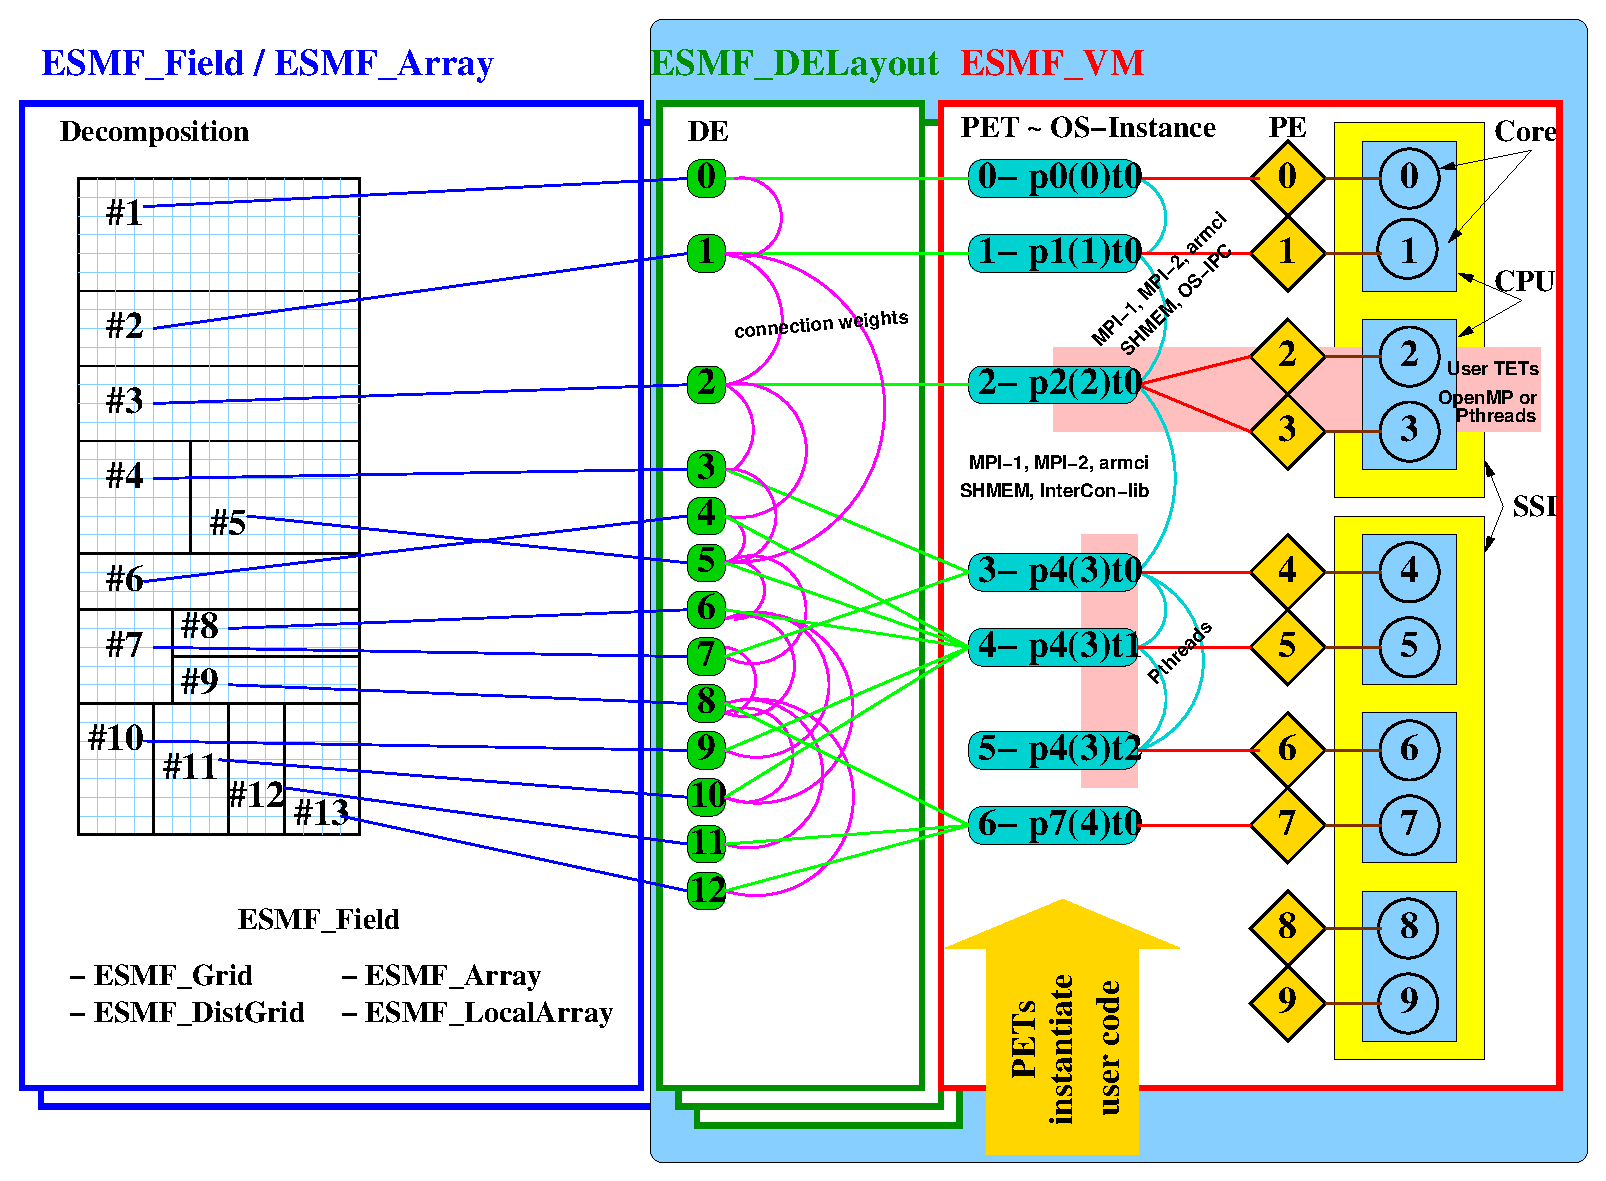
\includegraphics{VM_design.eps}}
%\end{center}


%{\bf Definition of terms used in the diagram}

%\begin{itemize}

%\item DE: Decomposition element.

%\end{itemize}
